%!TEX program = xelatex
%!BIB program = bibtex
\documentclass[cn,black,12pt,normal]{elegantnote}
\usepackage{float}
\usepackage{hyperref}
\usepackage{amsmath}
\usepackage{amsfonts}
\usepackage{amssymb}
\usepackage{siunitx}[=v2]
\usepackage{fancyhdr}
\usepackage{newtxtext}
\usepackage{algorithm}
\usepackage{algorithmic}
\newcommand{\uct}[1]{\textsuperscript{\textsuperscript{\cite{#1}}}}
\renewcommand{\tablename}{\textbf{Table}}
\renewcommand{\figurename}{Figure.}
\renewcommand{\refname}{References}
\renewcommand{\contentsname}{Contents}
\renewcommand{\versiontext}{Version: }
\renewcommand{\updatetext}{Update: }
\PassOptionsToPackage{no-math}{fontspec}
\lstset{basicstyle=\footnotesize\ttfamily\color[RGB]{50,0,130},numbers=none,frame=trBL}

\sisetup{mode=text}
\sisetup{range-phrase = \text{ \textasciitilde }}
\pagestyle{fancy}
\fancyhead[L]{School of Software Engineering, Tongji University}
\fancyhead[R]{Data Structure Projects}
\renewcommand{\headrulewidth}{1pt}

\title{Maze\\勇闯迷宫游戏}
\author{1951510\; 姜文渊}
\institute{\small \url{https://github.com/jwyjohn/Jwy_DataStructureHomework}}
\version{0.50}
\date{\today}

\begin{document}

\maketitle

\textbf{Data structure involved:} Stack, 2-d array

\textbf{Algorithms involved:} Depth first search, Minimum spanning tree

\tableofcontents

\newpage

\section{Introduction}

A maze is a path or collection of paths, typically from an entrance to a goal. Maze is also called Labyrinth, for some historical reasons.\uct{wiki:Labyrinth}

A maze can be both branching tour puzzles through which the solver must find a route, and simpler non-branching ("unicursal") patterns that lead unambiguously through a convoluted layout to a goal.\uct{wiki:Maze}

Due to the complexity of the maze, physical mazes have been built in large scales in history (e.g. The Egyptian labyrinth), for art or religion purposes. In that time, designing a Labyrinth is a challenging task since the systematic methods of generating mazes have not appeared before the development of graph theory and related algorithms.

Maze solving is the act of finding a route through the maze from the start to finish. Some maze solving methods are designed to be used inside the maze by a traveler with no prior knowledge of the maze, whereas others are designed to be used by a person or computer program that can see the whole maze at once.\uct{wiki:Maze} Solving a maze also takes effort, if given no assistance from modern computers and related theories.

In this project, the author built a demo for randomly generating mazes and solving them using related algorithms.

\begin{figure}[H]
    \centering
    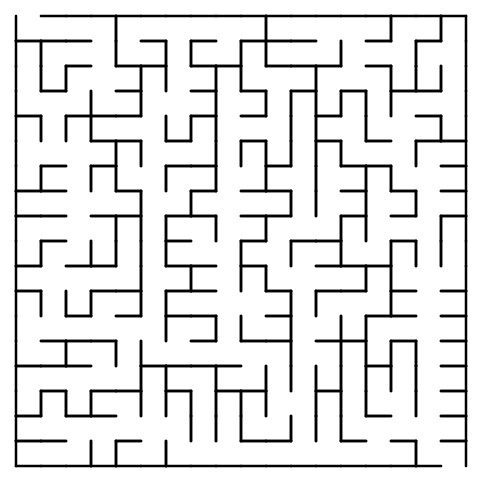
\includegraphics[width=0.5\linewidth]{image/tm.jpg}
    \caption{A typical maze}
\end{figure}

\section{Demostration}

\subsection{Compile and run the program}

On linux platform with \lstinline{make} and a \lstinline{g++} which supports C++ 11 Standard, just \lstinline{cd} to the \lstinline{./linux} and run \lstinline{make build}. The binary executable will be generated in the same directory named as \lstinline{a.out} or \lstinline{maze}, according to the configurations in the \lstinline{Makefile}. Use \lstinline{./a.out} or or \lstinline{./maze} to run the program.

\textbf{CAUTION} On windows platforms, the size of the shell \lstinline{cmd.exe} may not be suitable for big mazes, therefore it is recommended to compile and run the project on Linux platforms.

The program is an interactive shell, where you can input commands and get results.

\begin{figure}[H]
    \centering
    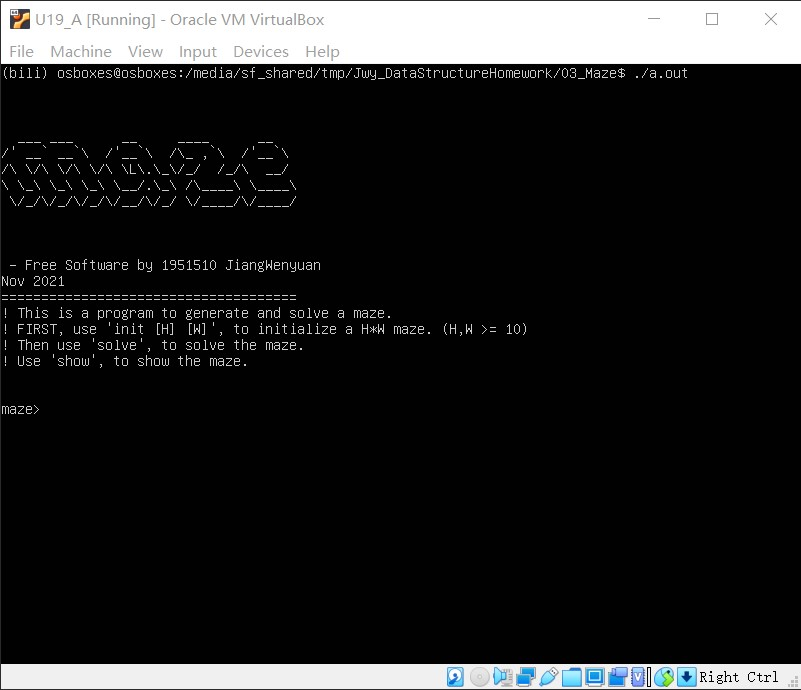
\includegraphics[width=0.7\linewidth]{image/m01.jpg}
    \caption{The user interface of the program}
\end{figure}

Usage of commands can be found on the main screen, and the \lstinline{help} command can give you information about theses commands.  All available commands is listed below.

\begin{enumerate}
    \item \lstinline{help} : Show help for a certain command.
    \item \lstinline{exit} : Exit the program.
    \item \lstinline{init [H] [W]} : Initialize a $H \times W$ maze, where $100 > H,W \geq 10$.
    \item \lstinline{show} : Print out the maze.
\end{enumerate}

\subsection{Generate a maze and solve it}

Type \lstinline{init 10 10} to generate a $10 \times 10$ maze. The generated maze is shown below. To print again the maze, use \lstinline{show}. We then type \lstinline{solve} to solve the maze.

\begin{figure}[H]
    \centering
    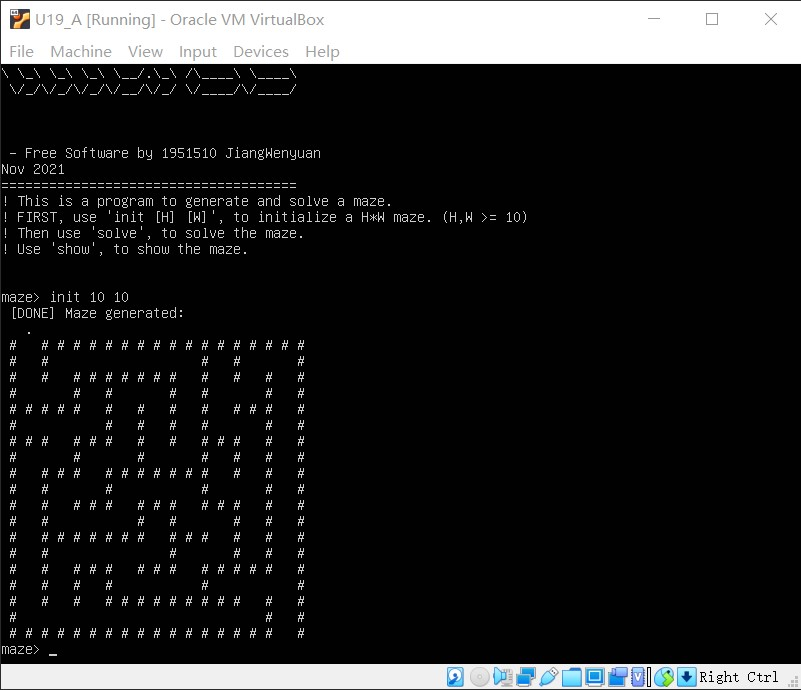
\includegraphics[width=0.7\linewidth]{image/m02.jpg}
    \caption{A $10 \times 10$ maze generated by the demo}
\end{figure}

\begin{figure}[H]
    \centering
    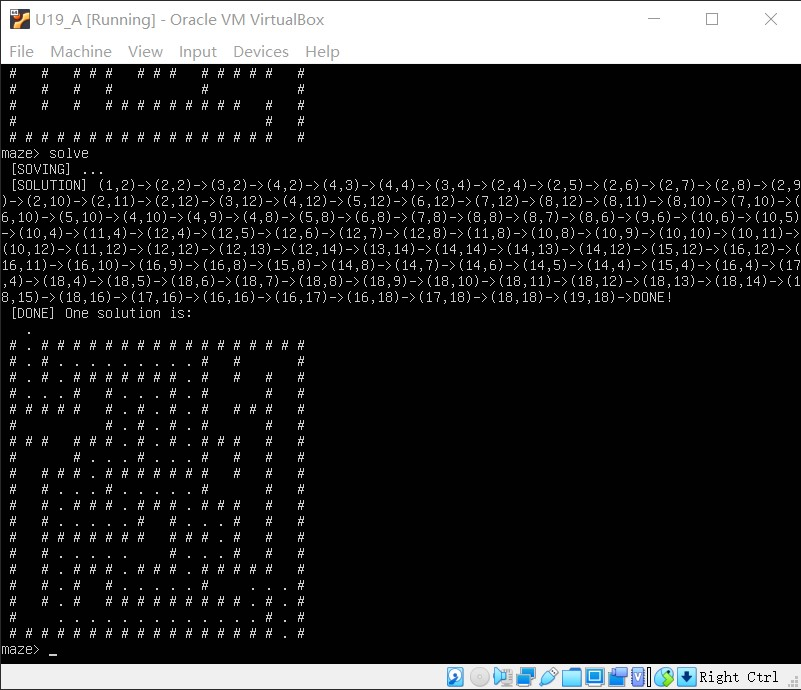
\includegraphics[width=0.7\linewidth]{image/m03.jpg}
    \caption{Use \lstinline{solve} to solve the maze}
\end{figure}

As can be seen on the two figures above, the maze is printed out with \lstinline{#} representing the walls. The entrance is on the left-top corner, while the exit is on the right-bottom corner.

The solution of a maze is shown both as sequence of \lstinline{(x,y)} points indicating the path to go, and in the graph form, with \lstinline{#} representing the walls and \lstinline{.} showing the solution path.

\begin{figure}[H]
    \centering
    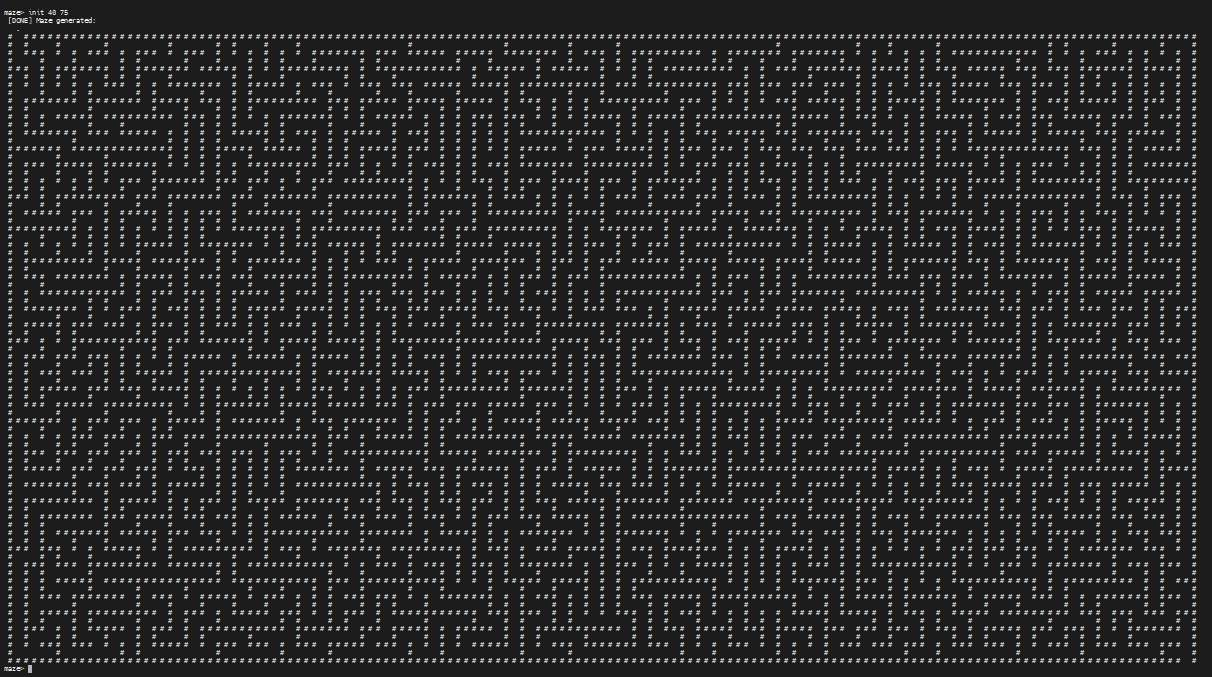
\includegraphics[width=0.9\linewidth]{image/m04.jpg}
    \caption{A $40 \times 75$ maze generated by the demo}
\end{figure}
\begin{figure}[H]
    \centering
    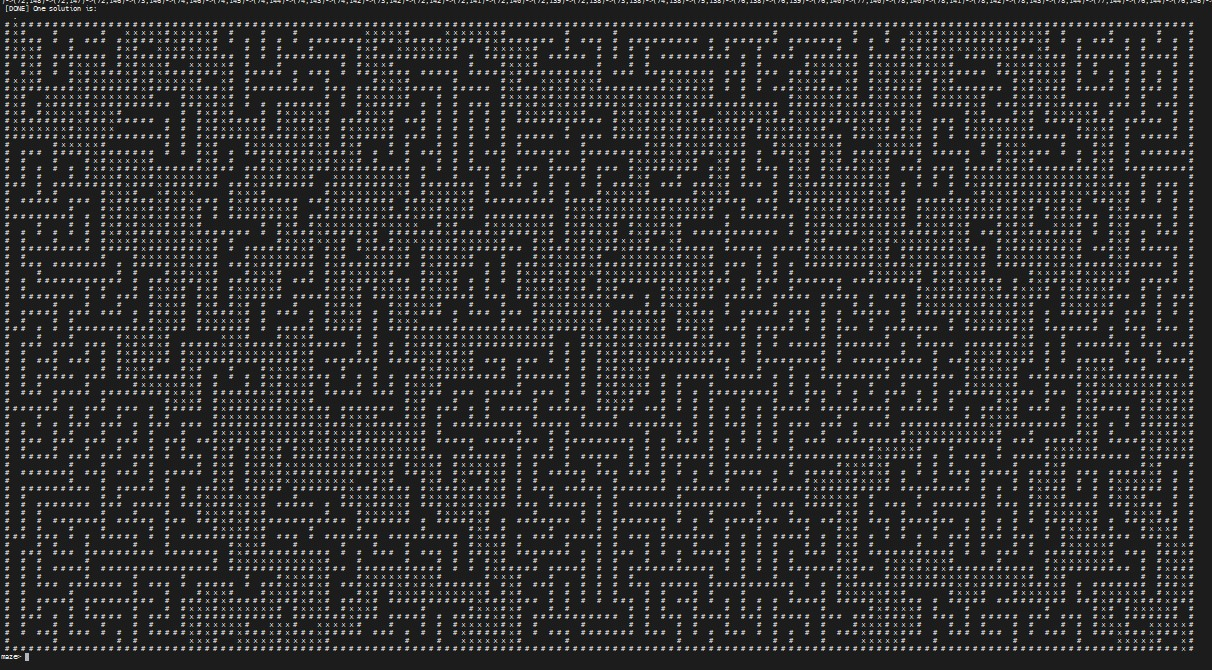
\includegraphics[width=0.9\linewidth]{image/m05.jpg}
    \caption{Solution of the maze above}
\end{figure}

We then used the same method to generate a $40 \times 75$ maze and solved it, with the results shown in the figure above. Note that to make the solution more claer, we used \lstinline{x} to represent the solution path in Figure 6.

\section{Generating and solving mazes}

\subsection{Use randomized spanning tree to generate a maze}

Graph theory based methods provide us with ways to generate mazes by seeing a 2-d array as nodes connecting with its neighbours (i.e. a 2-d grid). One of the most common ways of generating a maze is by generating a randomized spanning tree on the 2-d grid.

Minimum spanning trees algorithm, like the Kruskal's algorithm and the Prim's algorithm, can be used on a 2-d grid with random edge weight to give out a maze backbone. These algorithms need little or no modification to be adapted to the maze generation task. Typically, the time cost of these algorithms is $O(n\, log\, n)$, if using a heap to maintain the queue and an adjacent linked list for storing the graph.

Another method, the randomized depth first search, seems to have little connection with minimum spanning trees, but since the randomized depth first search on the given 2-d grid also produces a spanning tree, it can also be used to generate a maze. The implementation of the randomized depth first search can be done using a stack for backtracking, or can be done by recursive procedures. In this demo, the author choose randomized depth first search as the way of generating a maze.

However, randomized spanning trees have biases of various sorts: depth-first search is biased toward long corridors, while Kruskal's/Prim's algorithms are biased toward many short dead ends.\uct{wiki:Maze_generation_algorithm}


\subsection{Wilson's algorithm}

Wilson's algorithm\uct{wilson1996generating} is a kind of Loop-erased random walk, which can generate an unbiased sample from the uniform distribution over all mazes.

We begin the algorithm by initializing the maze with one cell chosen arbitrarily. Then we start at a new cell chosen arbitrarily, and perform a random walk until we reach a cell already in the maze—however, if at any point the random walk reaches its own path, forming a loop, we erase the loop from the path before proceeding. When the path reaches the maze, we add it to the maze. Then we perform another loop-erased random walk from another arbitrary starting cell, repeating until all cells have been filled.\uct{wiki:Maze_generation_algorithm}

\subsection{Use depth-first search to solve a maze}

To find a solution for a maze, depth-first search is one of the best choices, since it can provide a solution in relatively short time. The ordinary depth-first search is capable for randomly generated mazes, but for some extreame cases, some heuristic algorithm can be used to optimize the performance of ordinary depth-first search.

For a maze with more than one solution, there is a need to find a shortest path among the solutions. In this situation, depth-first search can have very poor performance, while the Breadth-first search can run averagely faster.

Searching algorithms have the computational complexity of ${\displaystyle O(|V|+|E|)}$, while depth-first search, if lucky enough, can find a way out in far less than this time.

\section{Notes on the source code}

\paragraph{The data structure of a maze} The following code defines several arrays and variables to store the maze.
\begin{lstlisting}[language = C++]
int w, h, start, end_p;
int M[1000][1000];
bool visited[1000][1000];
int R[1000][1000];
bool S_visited[1000][1000];
bool is_solved;
bool is_init = false;
\end{lstlisting}
The \lstinline{w} and \lstinline{h} are the width and height of the maze, and the \lstinline{M[1000][1000]} is the maze map. If \lstinline{M[i][j] == 0}, it means that the position \lstinline{(i,j)} is a wall, otherwise it is not a wall. After solving the maze, if \lstinline{(i,j)} is in the solution, \lstinline{M[i][j]} will be set to \lstinline{-1}.

\paragraph{Generation of the maze} The process of generating a maze consists of two major parts: \lstinline{int walkmaze(int x, int y, int n)} and \lstinline{int start_generate_maze()}.
\begin{lstlisting}[language = C++]
int walkmaze(int x, int y, int n)
{
	if (is_in_bound(x, y) && (!visited[x][y]))
	{
		R[x][y] = n;
		visited[x][y] = true;
		int di = rand() % 24;
		for (int i = 0; i < 4; i++)
		{
			walkmaze(x + 1 * dx[c[di][i]], y + 1 * dy[c[di][i]], n + 1);
		};
	};

	return 0;
};
\end{lstlisting}
The procedure \lstinline{int walkmaze(int x, int y, int n)} mainly dose the randomized depth first search, and the searching steps are recorded in the \lstinline{int R[1000][1000];}. Then in \lstinline{int start_generate_maze()}, the data in \lstinline{int R[1000][1000];} is converted to \lstinline{M[1000][1000]} to form a map.
\begin{lstlisting}[language = C++]
for (int i = 0; i <= w; i++)
	{
		for (int j = 0; j <= h; j++)
		{
			if (R[i][j] != 0)
			{
......
			};
		};
	};
	for (int i = 1; i <= 2 * w; i++)
	{
		for (int j = 1; j <= 2 * h; j++)
		{
			if (M[i][j] == 0)
			{
......
			}
		};
	};
......
	return 0;
\end{lstlisting}

For example, \lstinline{int R[1000][1000];} and \lstinline{M[1000][1000]} would look like this:
\begin{lstlisting}[basicstyle=\tiny\ttfamily]
M:
    #    9    #    #    #    #    #    #    #    #    #    #    #    #    #    #    #    #    #
    #    1    9    2    9    3    9    4    9    5    #   48    #   45    9   44    9   45    #
    #    #    #    #    #    #    #    #    #    9    #    9    #    9    #    9    #    #    #
    #   16    #    9    9    8    9    7    9    6    #   47    9   46    #   43    9   42    #
    #    9    #    9    #    #    #    #    #    #    #    #    #    9    #    #    #    9    #
    #   15    #   10    #   33    9   32    9   31    9   32    #   47    #   40    9   41    #
    #    9    #    9    #    9    #    #    #    9    #    9    #    9    #    9    #    #    #
    #   14    #   11    #   34    9   35    #   30    #   33    #   48    #   39    9   38    #
    #    9    #    9    #    9    #    #    #    9    #    9    #    #    #    #    #    9    #
    #   13    9   12    #   35    #   28    9   29    #   34    9   35    9   36    9   37    #
    #    9    #    #    #    #    #    9    #    #    #    #    #    #    #    #    #    9    #
    #   14    9   15    9   16    #   27    9   26    9   25    #   44    9   45    #   38    #
    #    #    #    #    #    9    #    #    #    #    #    9    #    9    #    #    #    9    #
    #   27    9   28    #   17    9   18    #   23    9   24    #   43    9   42    #   39    #
    #    9    #    #    #    #    #    9    #    9    #    #    #    9    #    9    #    9    #
    #   26    #   23    9   22    #   19    #   22    #   45    9   44    #   41    9   40    #
    #    9    #    9    #    9    #    9    #    9    #    9    #    #    #    #    #    #    #
    #   25    9   24    #   21    9   20    9   21    #   46    9   47    9   48    9   49    #
    #    #    #    #    #    #    #    #    #    #    #    #    #    #    #    #    #    9    #
R:
    #    #    #    #    #    #    #    #    #    #    #
    #    1    2    3    4    5   48   45   44   45    #
    #   16    9    8    7    6   47   46   43   42    #
    #   15   10   33   32   31   32   47   40   41    #
    #   14   11   34   35   30   33   48   39   38    #
    #   13   12   35   28   29   34   35   36   37    #
    #   14   15   16   27   26   25   44   45   38    #
    #   27   28   17   18   23   24   43   42   39    #
    #   26   23   22   19   22   45   44   41   40    #
    #   25   24   21   20   21   46   47   48   49    #
    #    #    #    #    #    #    #    #    #    #    #
\end{lstlisting}

\paragraph{Solution of the maze} The function used to solve the maze is \lstinline{int Solve(int x, int y, vector<pair<int, int>> sol)}, which is a recursive function to implement depth-first search.
\begin{lstlisting}[language = C++]
int Solve(int x, int y, vector<pair<int, int>> sol)
{
	if (!S_visited[x][y] && is_in_M(x, y) && M[x][y] != 0)
	{
		S_visited[x][y] = true;
		vector<pair<int, int>> tmp = sol;
		tmp.push_back({x, y});
		if (x == (2 * w - 1) && y == (2 * h - 2))
		{
			SOLUTION.push_back(tmp);
			is_solved = true;
		};
		for (int i = 0; i < 4; i++)
		{
			Solve(x + dx[i], y + dy[i], tmp); \\ recursive here
		};
	};
	return 0;
};
\end{lstlisting}
The results of the searching is stored in \lstinline{vector<vector<pair<int, int>>> SOLUTION;}, and later a function \lstinline{int calc_solution()} draws the solution to the map \lstinline{M[1000][1000]}.

Most of the code in \lstinline{main.cpp} is for processing the user's input, which is not so interesting.


\section{Discussion}

In this project, we implemented the demo of generating and solving a maze. The results of generated mazes are satisfying, and the computational complexity of generating a maze is $O(wh)$, which is consistent with the maze size. Solving the maze is based on the method depth-first search, which generally takes $O(wh)$ to find a solution.

The Wilson's algorithm mentioned above is orignally a method of generating randomized spanning trees at a very fast speed, and is published as \textit{Generating random spanning trees more quickly than the cover time}\uct{wilson1996generating}, which means that the generation of a $w \times h$ maze could cost less than $O(wh)$, which is counter-intuitive.

\bibliography{references}
\end{document}
